\chapter{Introduction\label{chapter:introduction}}

\ifpdf
    \graphicspath{{chapter_introduction/figures/Raster/}{chapter_introduction/figures/PDF/}{chapter_introduction/figures/}}
\else
    \graphicspath{{chapter_introduction/figures/Vector/}{chapter_introduction/figures/}}
\fi

Humans have been fascinated by the possibility of replicating their images into an artificial system since ancient Greece.
Some Greek myths, for example, tell of artificial entities who aid, through extraordinary actions, the men in combat.
According to a legend, the hero Cadmus (\textgreek{Κάδμος}), after founding Thebes, planted dragon teeth, which became artificial soldiers -- Figure~\ref{fig:cadmus}. Another noteworthy example can be found in the \emph{Argonautica} (\textgreek{Ἀργοναυτικά}), a poem written by \emph{Apollonius of Rhodes} (\textgreek{Ἀπολλώνιος Ῥόδιος}). The author narrates the myth of Talos (\textgreek{Τάλως}), an invulnerable artificial giant made of bronze. 
According to the myth, Talos was in charge to guard Crete against pirates and invaders and did not hesitate to plunge himself into the flames and heat it up to a very high degree before crashing into and burning his foes.
These synthetic beings were not just employed in war; in fact, examples of a companion automaton may be found in Latin literature. In this regard, Pūblius Ovidius Nāsō, known as Ovid, writes about the myth of Pygmalion who fell in love with a statue, \emph{Galatea}, he had crafted with his own hands -- Figure~\ref{fig:galatea}. In response to his prayers, the goddess Aphrodite brought Galatea to life.
\begin{figure}[t]
\centering
    \begin{subfigure}[b]{0.68\textwidth}
        \centering
        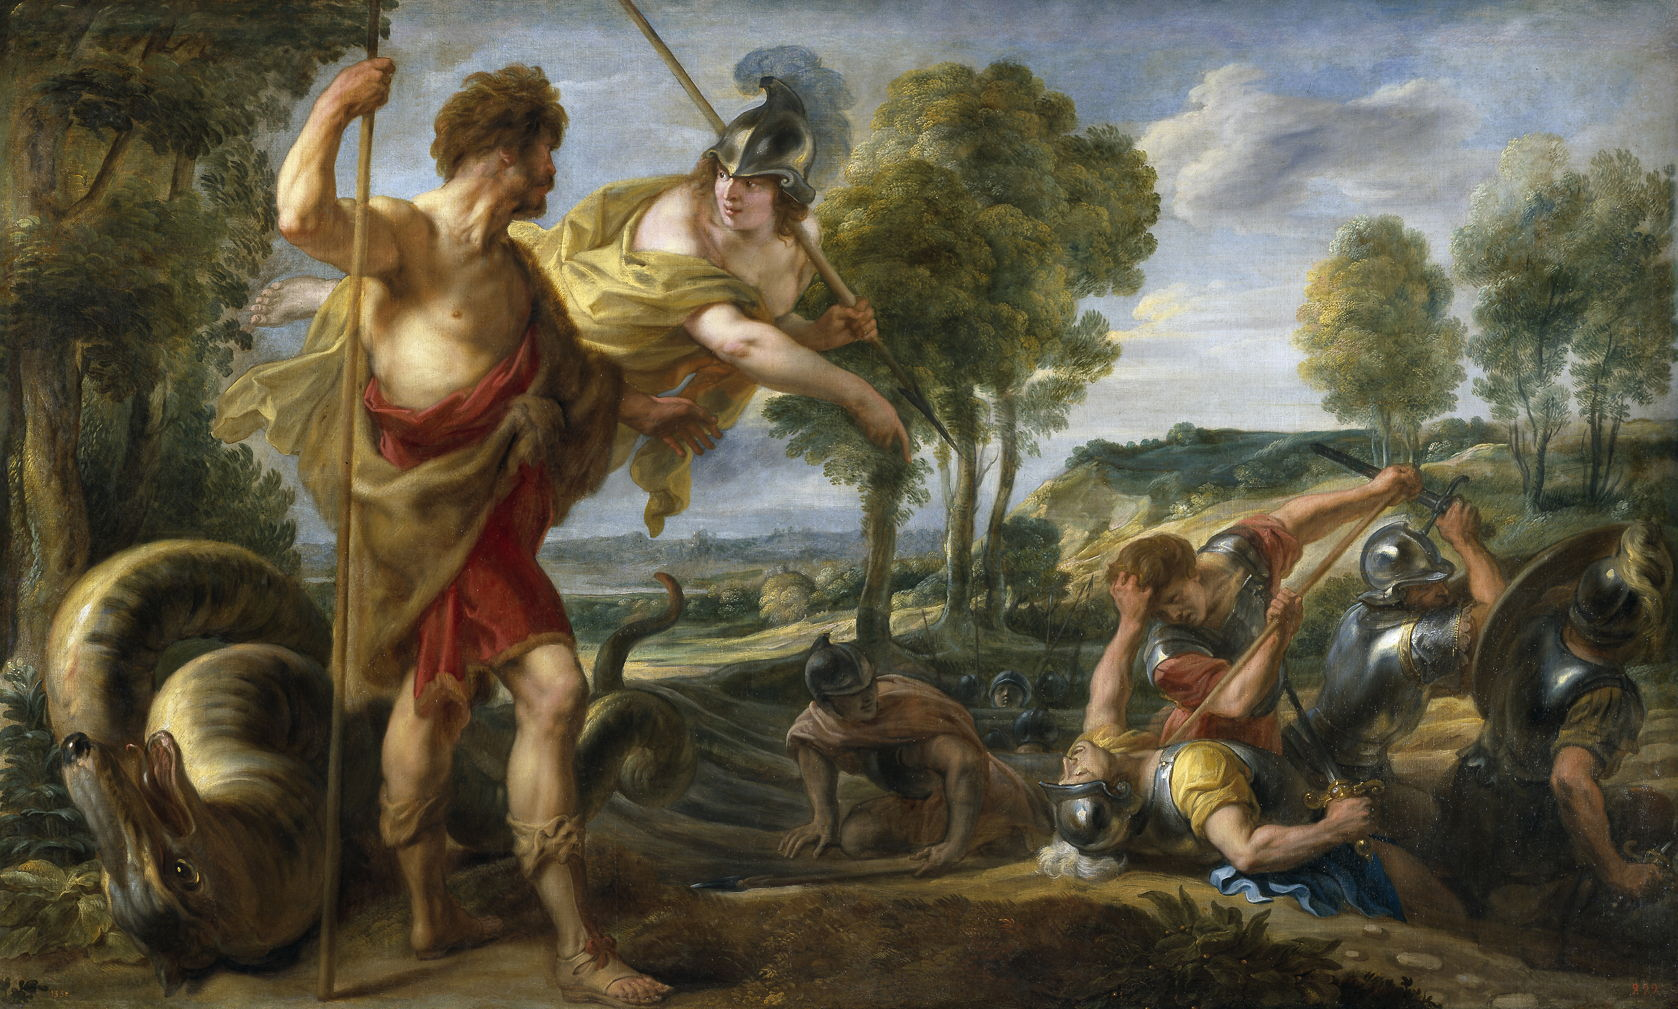
\includegraphics[height=6.25cm]{chapter_introduction/figures/cadmus.jpg}
        \caption{}
        \label{fig:cadmus}
    \end{subfigure}
    \hfill
    \begin{subfigure}[b]{0.31\textwidth}
        \centering
        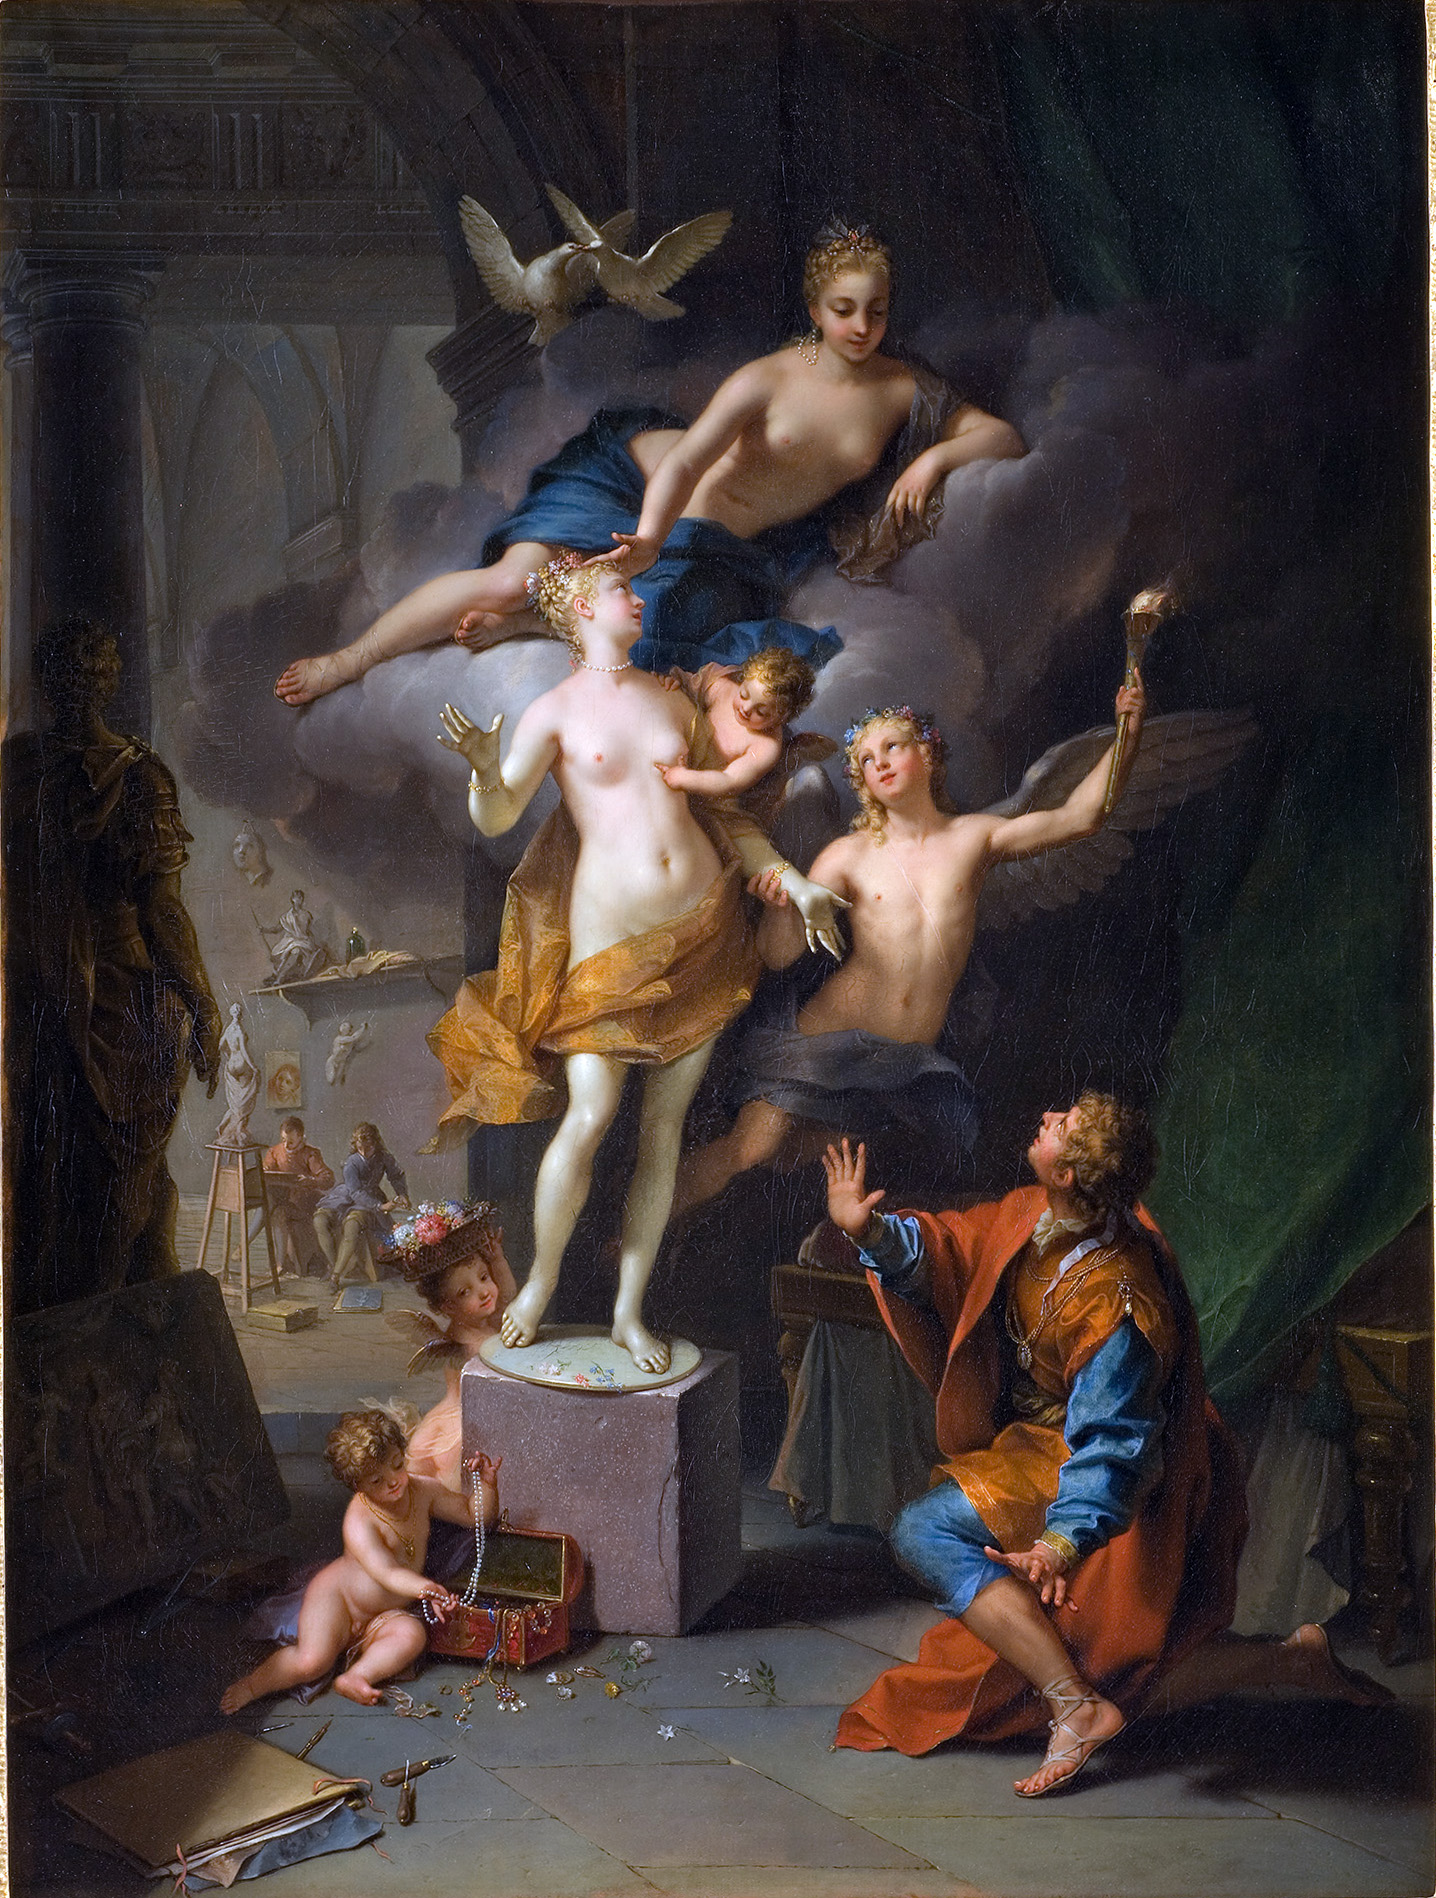
\includegraphics[height=6.25cm]{chapter_introduction/figures/galatea.jpg}
        \caption{}
        \label{fig:galatea}
    \end{subfigure}
    \caption[Art and robotics]{(a) Jacob Jordaens (1593–1678) - \emph{Cadmus and Minerva} (date not known). (b) Jean Raoux (1677-1734) – \emph{Pygmalion adoring his statue} (1717).}
	\label{fig:art}
\end{figure}
\begin{figure}[t]
\centering
 \begin{subfigure}[b]{0.27\textwidth}
        \centering
        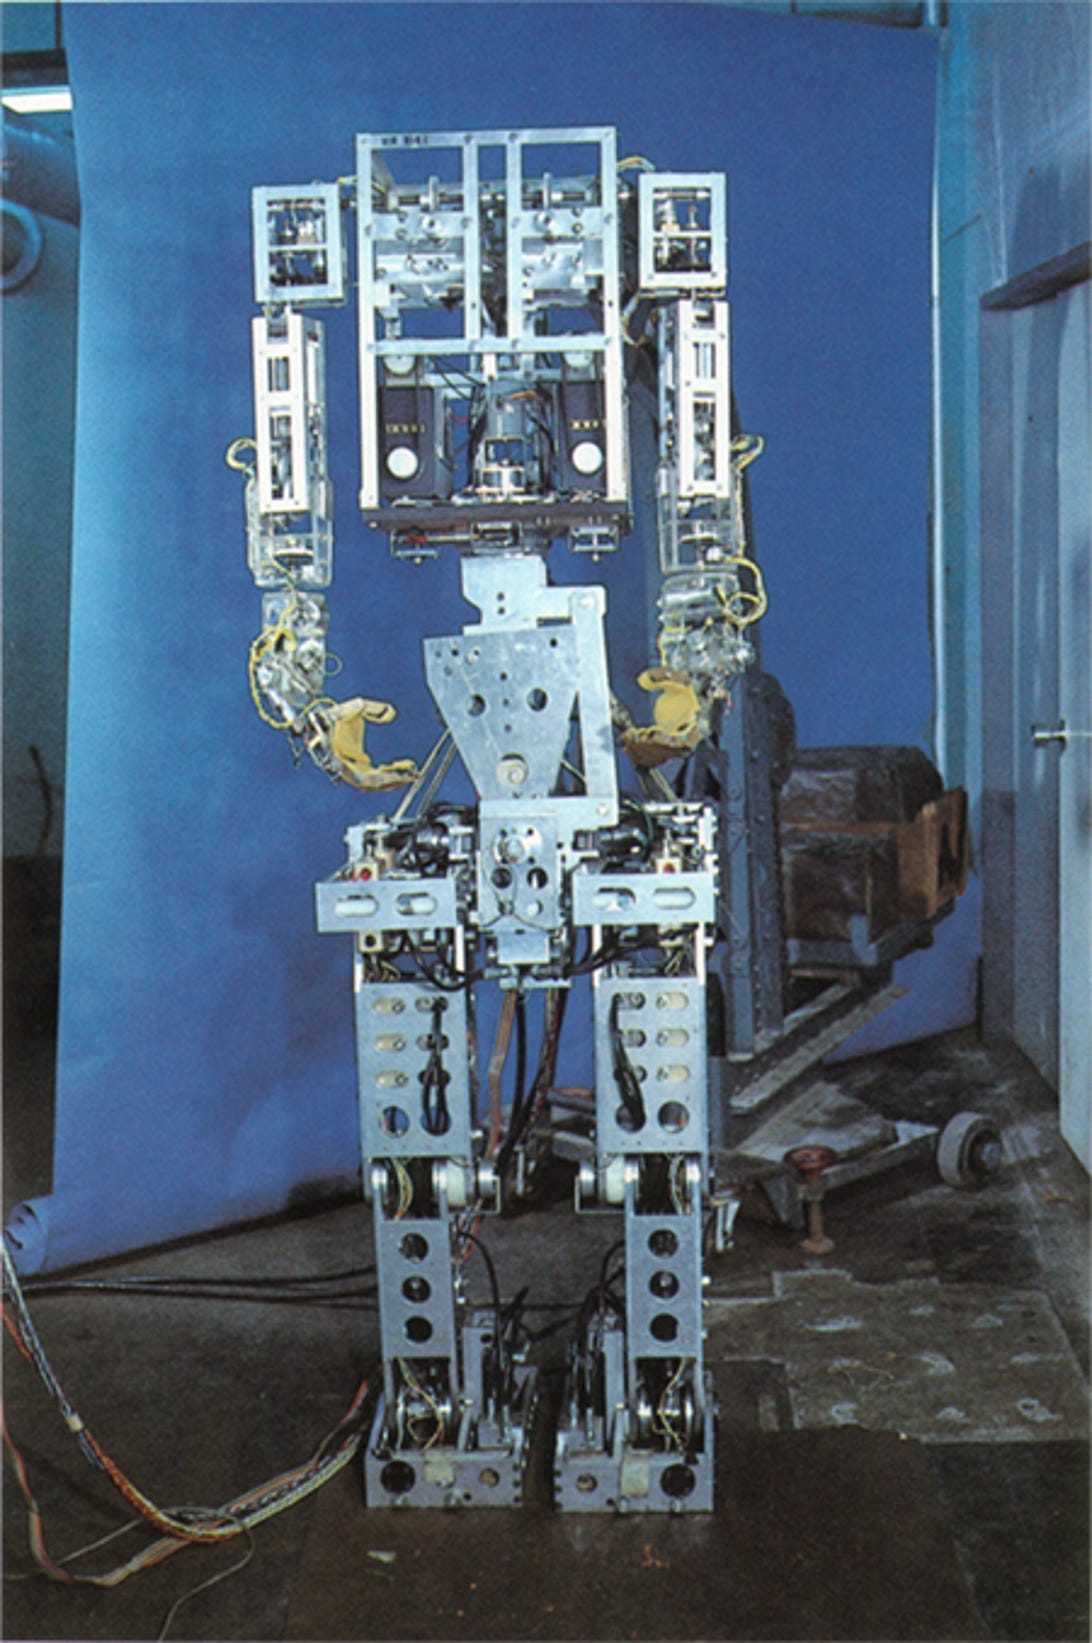
\includegraphics[height=6.2cm]{chapter_introduction/figures/WABOT-1.jpg}
        \caption{WABOT-1}
        \label{fig:wabot}
    \end{subfigure}
    \hfill
    \begin{subfigure}[b]{0.72\textwidth}
        \centering
        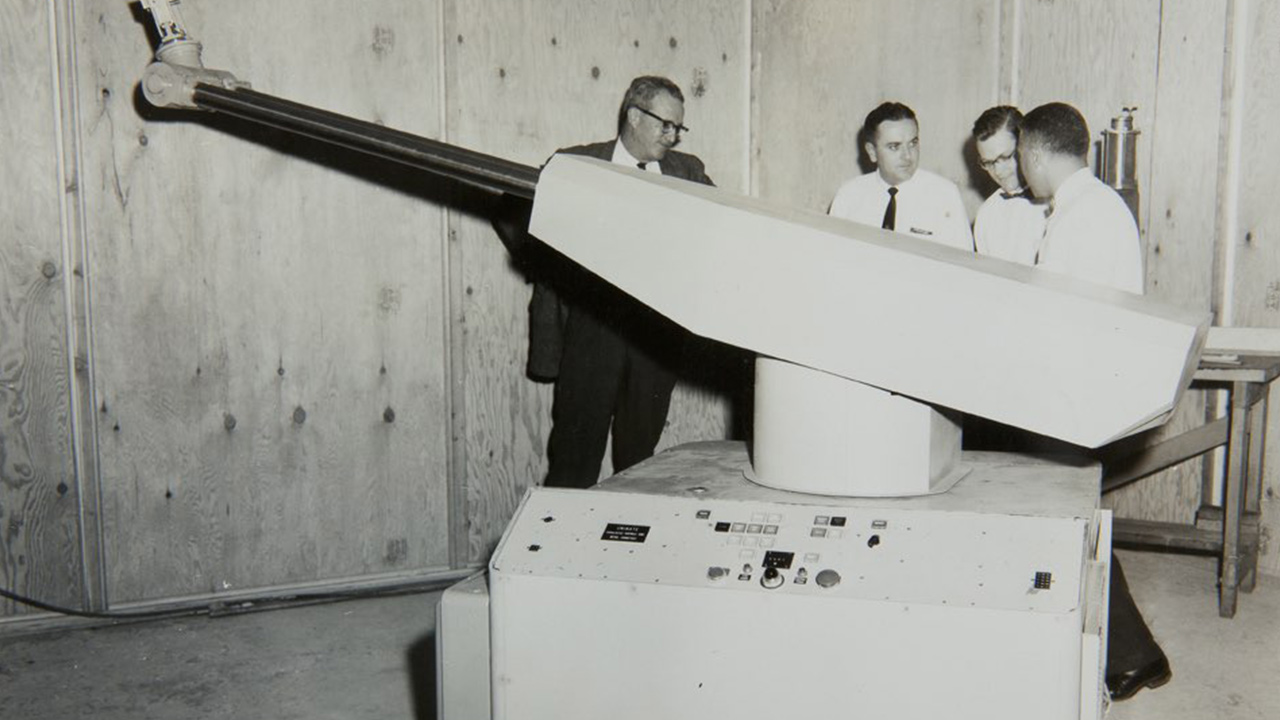
\includegraphics[height=6.2cm]{chapter_introduction/figures/unimate.jpeg}
        \caption{Unimate}
        \label{fig:unimate}
    \end{subfigure}
    \caption[WABOT-1 and Unimate]{ (a) The WABOT1 humanoid robot (image from \href{www.humanoid.waseda.ac.jp/booklet/kato\_2.html}{\texttt{www.humanoid.waseda.ac.jp/booklet/kato\_2.html}}).  (b) A picture of the Unimate robot (image taken from \href{https://latestnews.plus/the-film-like-story-of-the-first-real-robot-unimate-in-history/}{\texttt{https://latestnews.plus/the-film-like-story-of-the-first-real-robot-unimate-in-history/}}).}
\end{figure}
\par
It takes a long time to go from folklore to a documented project of an autonomous system. Given that the first one dates around 1495 when \emph{Leonardo da Vinci} designed the \emph{mechanical knight}, known as \emph{Leonardo's robot}. The project was probably based on Leonardo's concept of the ideal human body proportions represented in the \emph{Virtuvian Man} drawing. The first working android was built only about three centuries later by \emph{Jacques de Vaucanson} in 1738.
Jacques de Vaucanson's work can be seen as a bridge from an age in which artificial creatures were exclusively restricted to legends or projects, to another in which the ideal of developing artificial mechanical systems had become a reality.
This was noticed by the Italian writer \emph{Ippolito Nevio} who states in \emph{Storia Filosofica dei Secoli Futuri} that the invention of automata is the most important goal reached in the history of mankind.
\par
The term robot was coined by the Czech writer Karel Čapek, who used it for the first time in his play \emph{The Universal Robots of Rossum} to characterize an artificial worker. The worldwide success of Čapek's play helped the term \emph{robot} to gain a vogue. Nowadays, the word robot has been incorporated into practically every language.
\par
It is interesting to note that robots have had a human aspect since antiquity; yet, the first contemporary robots were used in industries and were not humanoid. The first industrial robot, \emph{unimate} (Figure~\ref{fig:unimate}), was constructed in 1959, while the first machine capable of human-like walking arrived only 14 years later in 1973. Its name was WABOT-1 (WAseda roBOT)~\citep{Takanishi2019HistoricalAsia} -- Figure~\ref{fig:wabot}. WABOT-1 weighs around $\SI{130}{\kilo \gram}$ and is powered by 11 hydraulically driven joints. Walking is accomplished by segmenting the motion and storing the associated joint references in the robot's \emph{computer}. An analog circuit attempts to match the reference joint position with the one measured by a potentiometer. Despite more than five decades since the first walking humanoid robot, bipedal locomotion remains an open problem. The complexity of the robot dynamics, the unpredictability of its surrounding environment, and the low efficiency of the robot actuation system are only a few problems that complexify the achievement of robust robot locomotion. As a result, to cope with the difficulty, researchers were driven to design simpler models~\citep{Kajita2001,vukobratovic2004zero,Pratt2006,Englsberger2011} that are only valid under strict assumptions. In this context, the definition of a hierarchical architecture composed of several layers was a common approach to achieve online humanoid robot control during the DARPA Robotics Challenge~\citep{Spenko2018TheRescue}. In this context, each layer assumes a particular robot model, and it provides the references for the inner layer by processing the inputs from the robot, the environment, and the outputs of the outer layer.
\par
This thesis explores the hierarchical control architecture and focuses on various model-based controllers for time-critical humanoid robot motion control. Depending on the desired objective, we vary the considered models from simplified to complete robot dynamics.
\par
In Sections~\ref{sec:icub} and \ref{sec:talos}, we briefly describe the technological resources used for the experimental validation of the thesis developments: \emph{iCub} and \emph{TALOS humanoid robots}. Section~\ref{sec:notation} introduces the notation used in the thesis 

\section{The iCub Humanoid Robot\label{sec:icub}}

\begin{figure}[tpb]
\centering
    \begin{subfigure}[b]{0.48\textwidth}
        \centering
        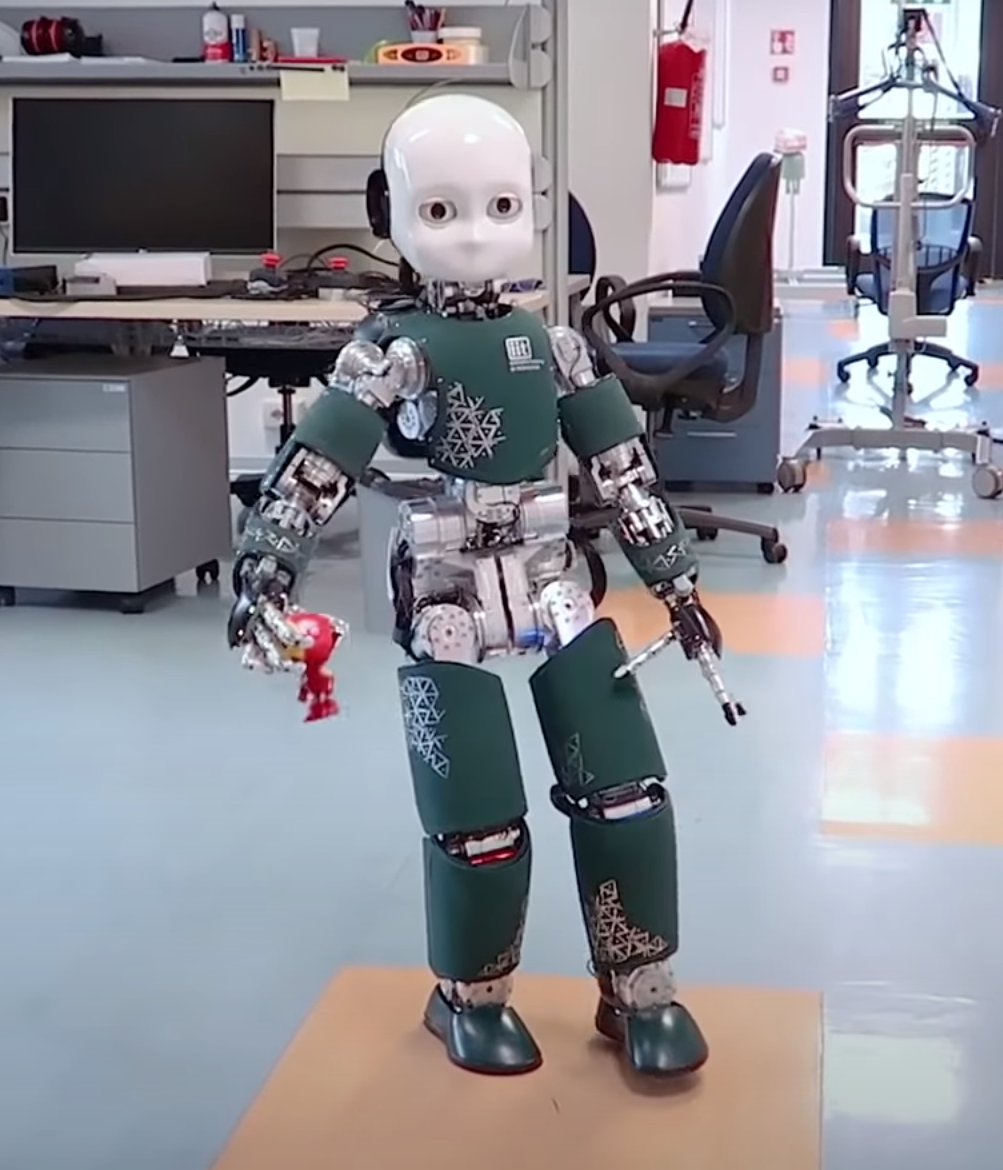
\includegraphics[width=\textwidth]{chapter_introduction/figures/iCubGenova04.png}
        \caption{The iCub v2.7 robot}
        \label{fig:iCubGenova04}
    \end{subfigure}
    \hfill
    \begin{subfigure}[b]{0.48\textwidth}
        \centering
        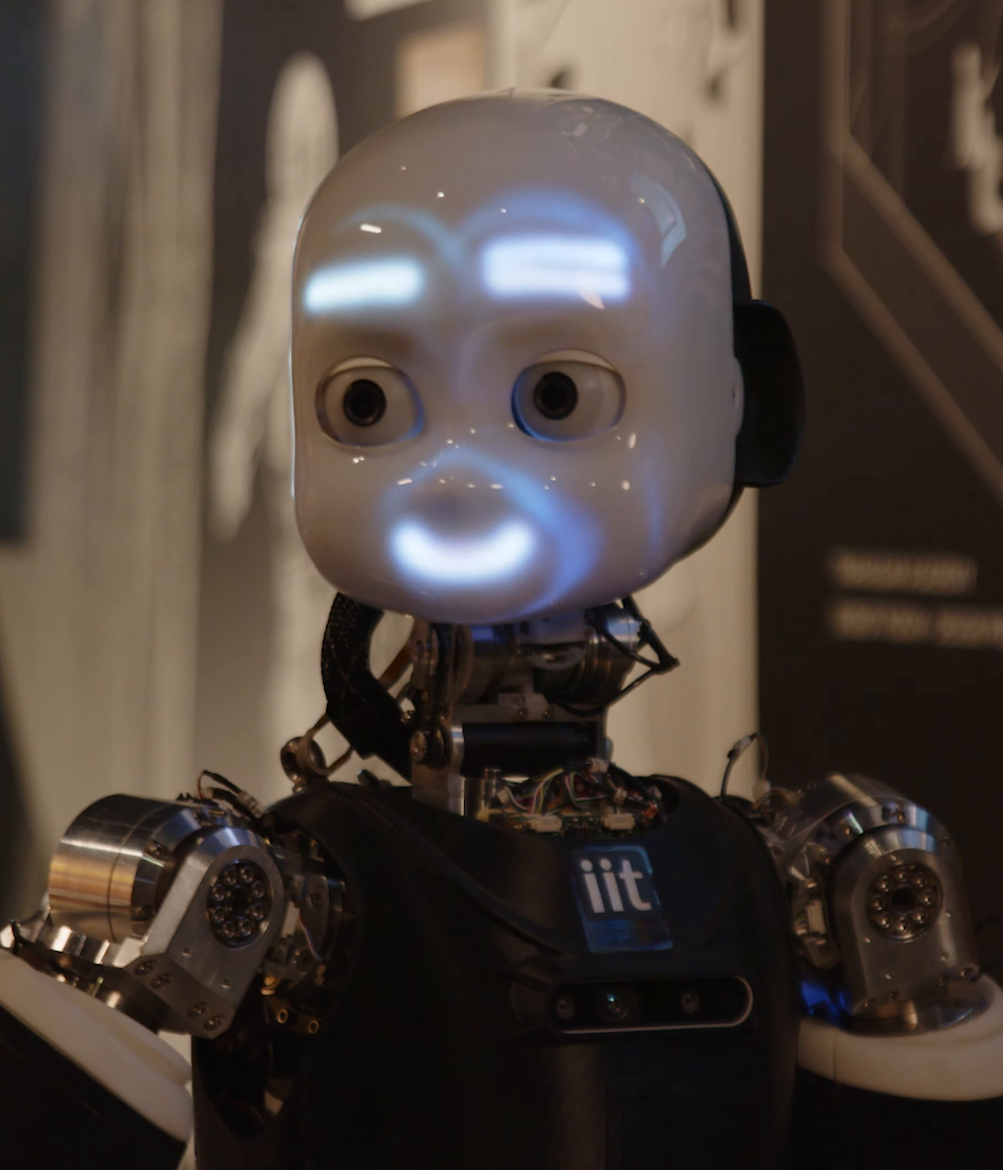
\includegraphics[width=\textwidth]{chapter_introduction/figures/iCubGenova09.png}
        \caption{The iCub v3 robot}
        \label{fig:iCubGenova09}
    \end{subfigure}
    \caption{The two versions of the iCub humanoid robot.}
	\label{fig:icub}
\end{figure}


\begin{figure}[tpb]
\centering
    \begin{subfigure}[b]{0.48\textwidth}
        \centering
        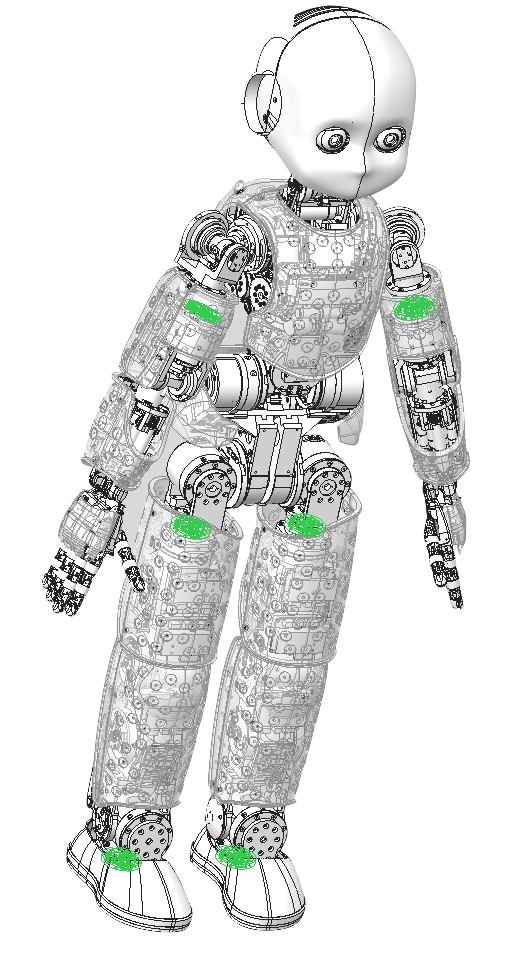
\includegraphics[height=\textwidth]{chapter_introduction/figures/icub_ft.png}
        \caption{Distribution of the six-axis force-torque}
        \label{fig:iCubGenova04_ft}
    \end{subfigure}
    \hfill
    \begin{subfigure}[b]{0.48\textwidth}
        \centering
        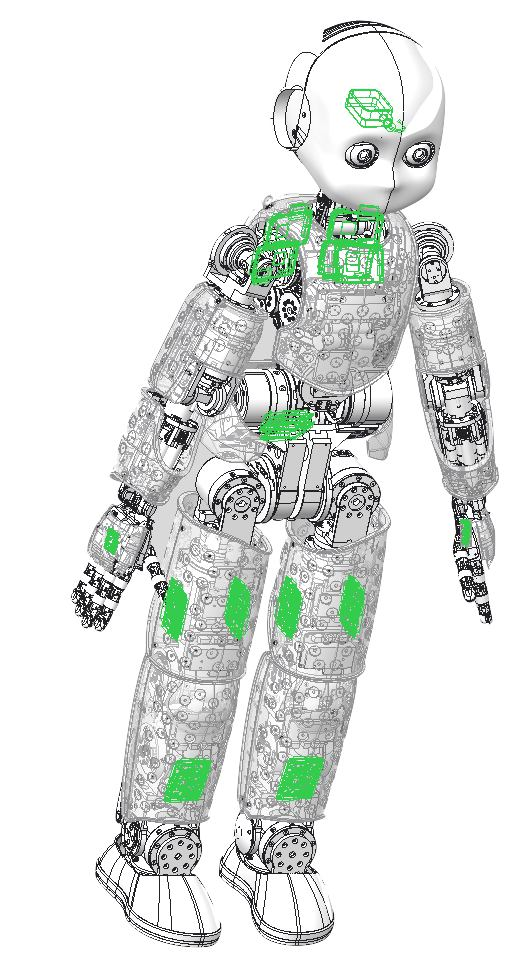
\includegraphics[height=\textwidth]{chapter_introduction/figures/icub_imu.png}
        \caption{Distribution of the inertial sensors}
        \label{fig:iCubGenova04_imu}
    \end{subfigure}
    \caption[FT and IMU distribution on iCub v2.7]{Distribution of the six embedded six-axis force-torque sensors (a) and of the inertial sensors (b) on iCub v2.7.}
	\label{fig:iCubGenova04_sensors}
\end{figure}

The iCub Humanoid Robot is an open source state-of-the-art robotic platform created as part of the European project RobotCub~\citep{Tsagarakis2007,Natale2017,Parmiggiani2012,Metta2010} at the Italian Institute of Technology.
The iCub has been regularly updated with upgrades and new features since its first release in 2006. More than 40 partnering institutions in Europe, Asia, and the United States have received copies of iCub. 

Because innovations are constantly issued and integrated into the many iCubs, all robot copies have distinct features based on their release date, the maintenance upgrades conducted over the years, and the individual customization of each iCub. The algorithms discussed in the thesis have been tested on two versions of the iCub robots, namely iCub v2.7 and iCub v3. Section~\ref{sec:icub2.7} presents the characteristics of iCub v2.7, while Section~\ref{sec:iCub3} introduces iCub v3. 

\subsection{The iCub v2.7 robot\label{sec:icub2.7}}

Figure~\ref{fig:iCubGenova04} depicts the iCub humanoid robot v2.7, which is $\SI{104}{\centi\meter}$ tall and weighs $\SI{33}{\kilo\gram}$. It has 54 degrees of freedom in total, including those in the hands and eyes. Only 23 joints are used for locomotion and are distributed as follows: 4 joints in the arm, 3 of which in the shoulder and one in the elbow, 3 joints in the torso, and 6 joints in each leg. 
The torso and shoulder joints are mechanically coupled and driven by tendon mechanisms. All 23 joints are powered by brushless electric motors equipped with Harmonic Drive transmissions with a reduction ratio of 1/100.

A series of electronic boards known as 2FOC, EMS, and MC4Plus operate the iCub motors. The 2FOC boards use an incremental optical encoder positioned on the motor shaft to regulate the magnetic flux of a brushless motor by setting a reference PWM (Pulse Width Modulation). The EMS boards, on the other hand, are linked to the 2FOC boards and implement three control strategies, namely position, velocity, and torque control. The electronic boards are connected through an Ethernet network in daisy chain.
\par
A three-degree-of-freedom accelerometer and three-degree-of-freedom gyroscopes are included on each motor control board. In addition, the robot's head is equipped with a full-fledged Inertial Measurement Unit, which includes a 3 DOF magnetometer, accelerometer, and gyroscope. Figure~\ref{fig:iCubGenova04_imu} shows how these designs offer the iCub v2.7 with a large amount of distributed inertial sensing, which has been exploited for precise calibration in~\citep{Guedelha2016Self-calibrationMeasurements}.
\par
Differently from other state-of-the-art robots \citep{Englsberger2015OverviewTORO,Stasse2017TALOS:Applications}, the iCub humanoid robot v2.7 does not mount pure torque sensors on the joints. As a consequence, the internal joint torques cannot be directly measured. However the robot is equipped with 6 inertial six-axis force-torque sensors - Figure~\ref{fig:iCubGenova04_ft}. Four of them are attached to the base of each limb, while two are mounted on the robot's ankles. The location of these sensors enables the estimation of internal joint torques and external force-torque, as described in~\citep{Fumagalli2012} for a single limb and in \citep[Chapter~4]{Traversaro2017ModellingDynamics} for the whole-body case.
\par
Finally, the robot head is equipped with a 4$^{\text{th}}$ generation Intel\textsuperscript{\textregistered} Core i7@1.7GHz and 8GB of RAM running Ubuntu Linux. Finally, the connection to the robot can be established through an Ethernet cable or thought a standard 5GHz Wi-Fi network.

\begin{figure}[t]
\centering
    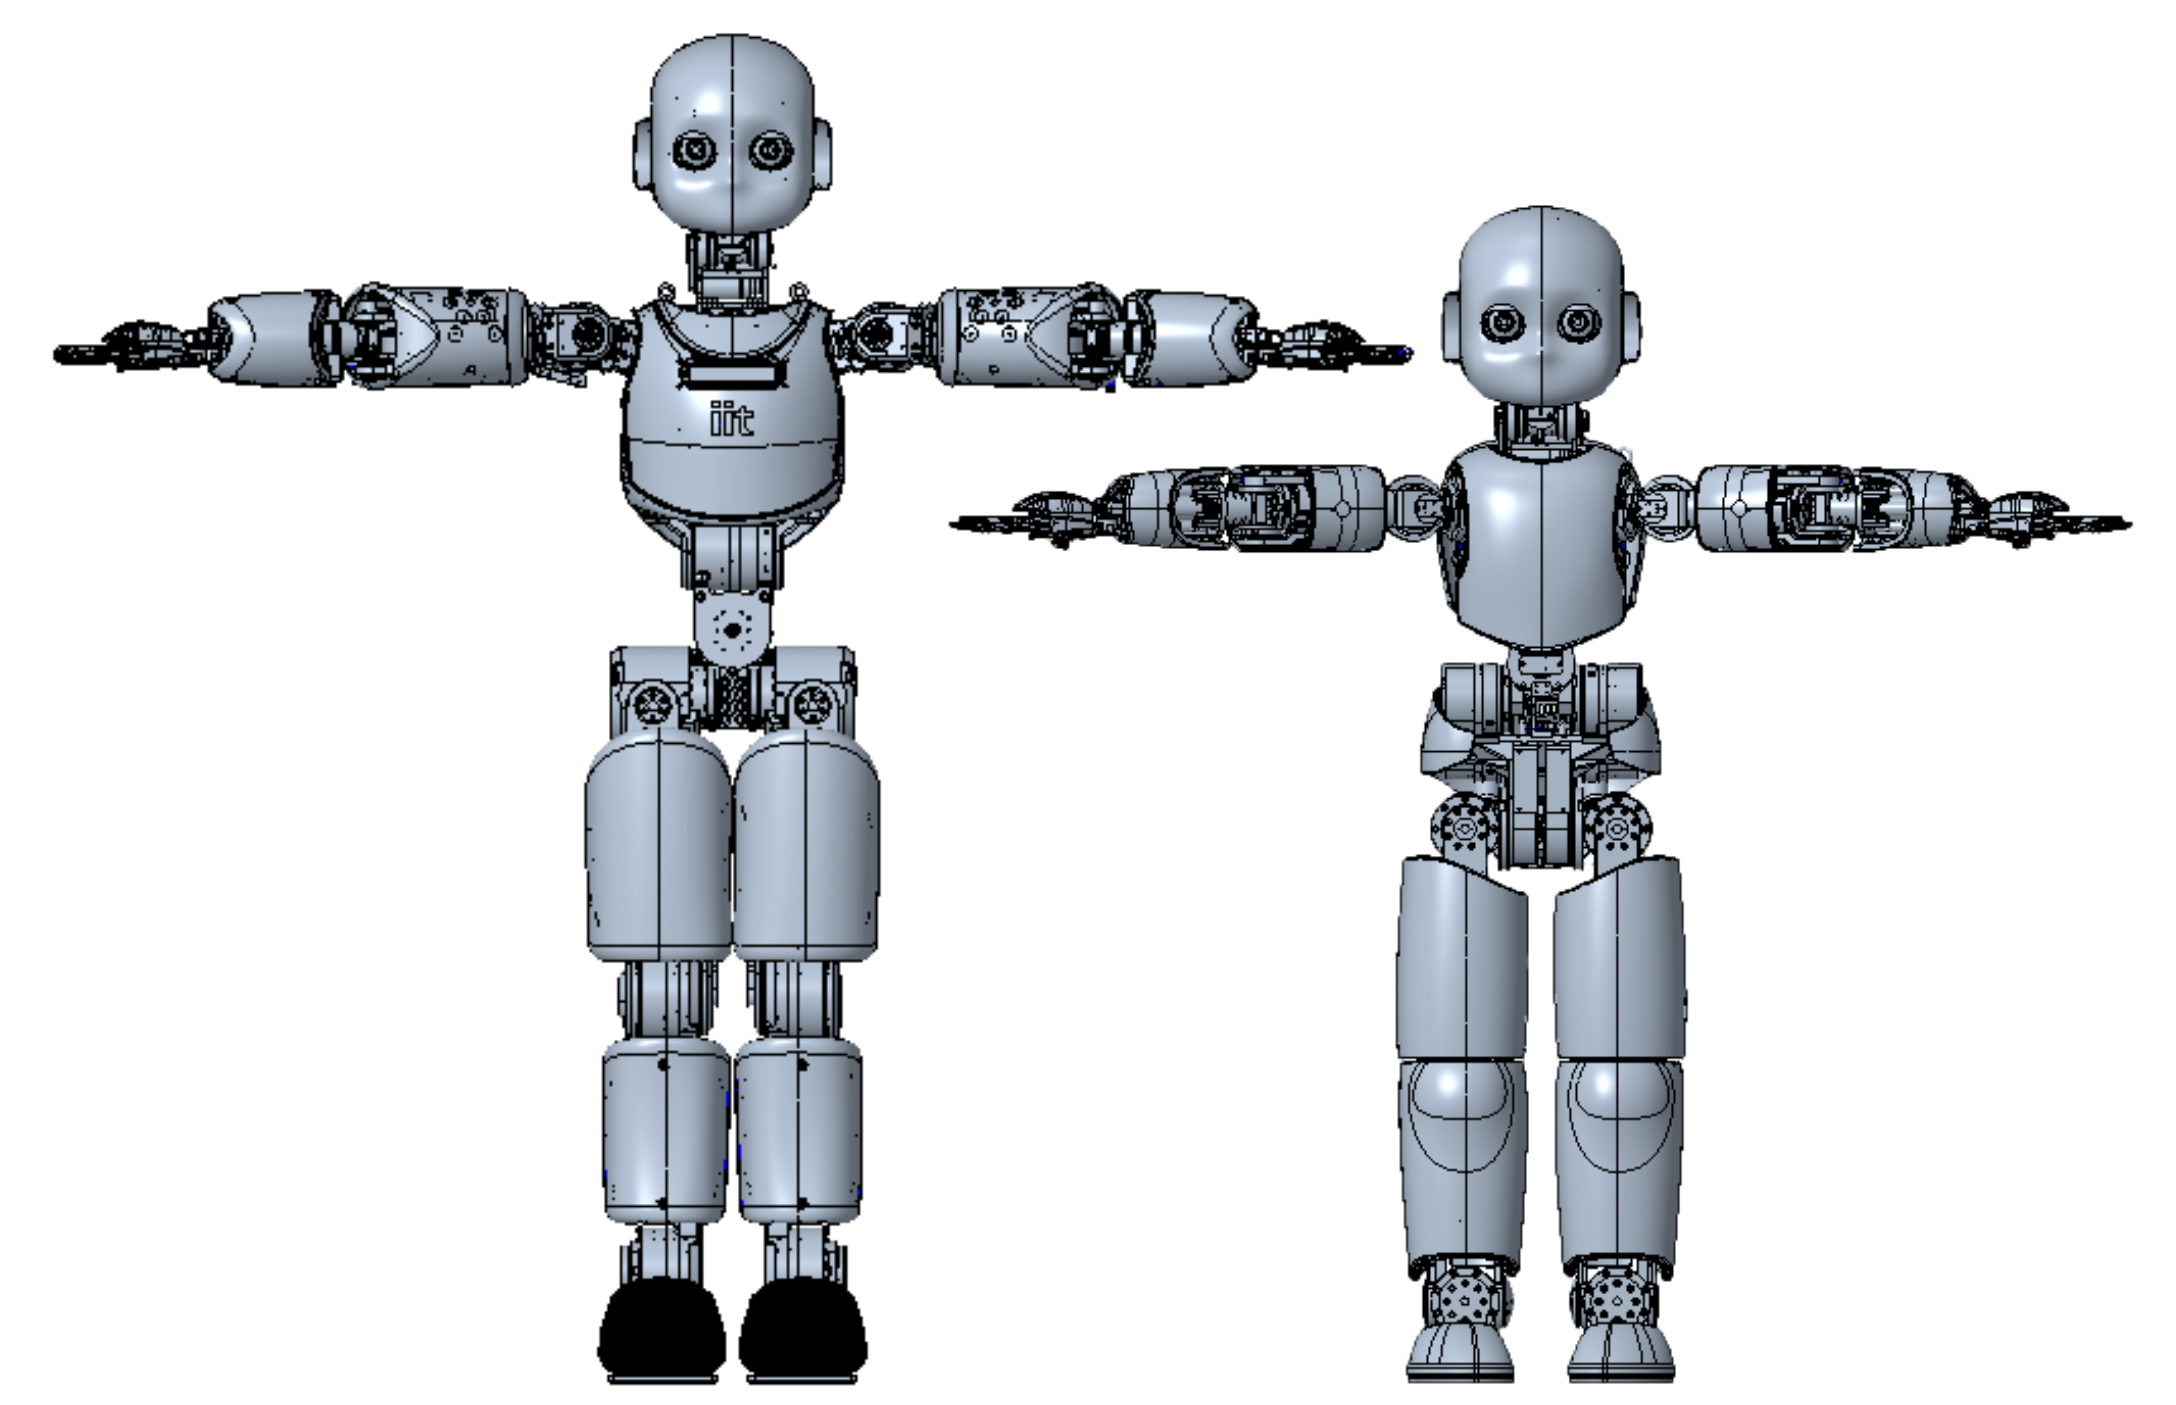
\includegraphics[width=\textwidth]{chapter_introduction/figures/icub_comparison.png}
    \caption{The iCub3 robot side to side to the classical iCub v2.7.
    \label{fig:icub_comparison}}
\end{figure}


\subsection{The iCub v3 robot} \label{sec:iCub3}
The iCub v3 humanoid robot, depicted in Figure \ref{fig:iCubGenova09}, is a state-of-the-art robotic platform developed at the Italian Institute of Technology and can be seen as an evolution of the iCub v2.7 presented in Section~\ref{sec:icub2.7}. 
\par
The iCub v3 humanoid robot is larger than a traditional iCub v2.7 platform, standing $\SI{25}{\centi\meter}$ higher and weighing $\SI{22}{\kilo\gram}$ heavier. The robot is $\SI{125}{\centi\meter}$ tall and weighs $\SI{52}{\kilo\gram}$. Figure \ref{fig:icub_comparison} shows the different dimensions of the two platforms.
The greater weight necessitates more powerful leg motors. As a consequence of the increased size of the actuators, a new approach to the knee and ankle pitch joints was necessary. Specifically, instead of being on the same axis, the motor and actuator are separated and linked by belts. Similarly to iCub v2.7, the iCub v3 robot possesses in total 54 degrees of freedom, including those in the hands and the eyes, and only 23 joints are used for locomotion. However, unlike iCub v2.7, the torso and shoulder joints are not tendon-driven. In fact, the joints are directly connected to the motor shaft throughout the serial direct mechanisms. This provides for a larger range of motion and mechanical toughness.
All 23 joints used for locomotion are powered by brushless three-phase electric motors equipped with Harmonic Drive transmissions. 
Each foot is made up of two rectangular parts, each measuring $\SI{25}{\centi\meter}$ in length and $\SI{10}{\centi\meter}$ in width.
\par
Similarly to iCub v2.7, iCub v3 is equipped with a vast array of sensors, including accelerometers, gyroscopes, and force/torque sensors. Six six-axis force/torque (F/T) sensors are included in the iCub. Two are placed on each shoulder and two are attached to each foot, linking the two portions of the feet to the ankle assembly. The readouts of the F / T sensors are used to estimate the internal joint torques and the external force-torque, as presented in \citep[Chapter~4]{Traversaro2017ModellingDynamics}.

\subsection{Software infrastructure}
A computer infrastructure is required to control the robot. To
this end, the Yet Another Robot Platform (YARP) middleware~\citep{Metta2006} is exploited. YARP is an open-source multi-platform middleware whose main purpose is to allow communication between the applications (modules), which can run on different computers. More specifically, YARP is a set of libraries, protocols, and tools to keep modules and devices cleanly decoupled. Indeed, it provides an abstraction layer to interact with physical devices, such as joint encoders and F/T sensors, independently of their actual implementation. Moreover, sensor acquisition and motor controllers are provided through YARP interfaces.
\par
Along with the YARP middleware, we took advantage of the iDynTree library~\citep{Nori2015} to design the controllers. iDynTree is a library of robot dynamics algorithms for control, estimation, and simulation. It is specifically designed for free-floating robots, but it is also possible to use it with fixed-base robots. It is written in \texttt{C++}, with Python and MATLAB interfaces. iDynTree contains support for reading and writing \texttt{URDF} files, making it possible to use it with any type of robot described by an \texttt{URDF}.
\par
Rapid prototyping is achieved thanks to iDyntree interfaces, which can be easily integrated into off-the-shelf Python libraries and Simulink and MATLAB toolbox. Controller prototyping also takes advantage of the Gazebo simulation environment \citep{Koenig04}. Gazebo is an open source simulator that can efficiently simulate complex multibody systems. The interface between the controller algorithms and the simulated version of the robot is handled through the corresponding YARP plugins \citep{MingoHoffman2014}. The plugins make the algorithm implementation transparent. In fact, they allow testing of the very same software on both the simulator and the real robot.
\begin{figure}[t]
\centering
    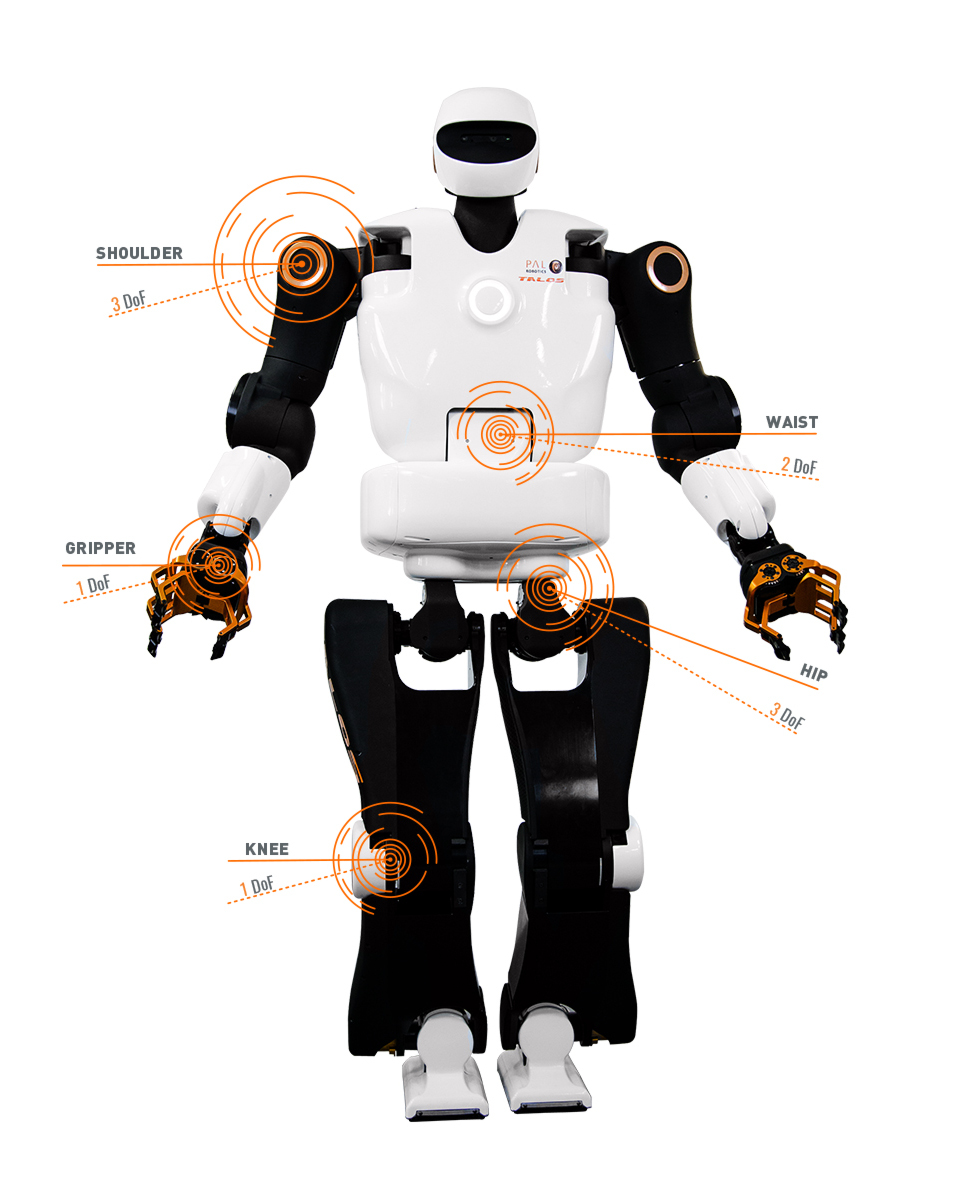
\includegraphics[width=0.6\textwidth]{chapter_introduction/figures/TALOS_FRONT.jpg}
    \caption[TALOS humanoid robot]{TALOS humanoid robot. Image taken from~\href{https://pal-robotics.com/robots/talos/}{\texttt{https://pal-robotics.com/robots/talos/}}
    \label{fig:talos}}
\end{figure}

\section{The TALOS Humanoid Robot\label{sec:talos}}
TALOS is a state-of-the-art humanoid robot that integrates the latest cutting-edge robotics technology~\citep{Stasse2017TALOS:Applications} designed and developed by PAL-Robotics -- Figure~\ref{fig:talos}.
By construction, the robot is capable of interacting with a human environment and targeting industrial applications. 
Since its release, several versions of TALOS have been produced, the following is the detailed description of \emph{Pyr\`{e}ne}, the first robot in the TALOS series built by PAL-Robotics, currently available and maintained by the Gepetto group at LAAS-CNRS in Toulouse. The content of this section is inspired by the official presentation of the robot available in \cite{Stasse2017TALOS:Applications}.
\begin{figure}[tpb]
\centering
    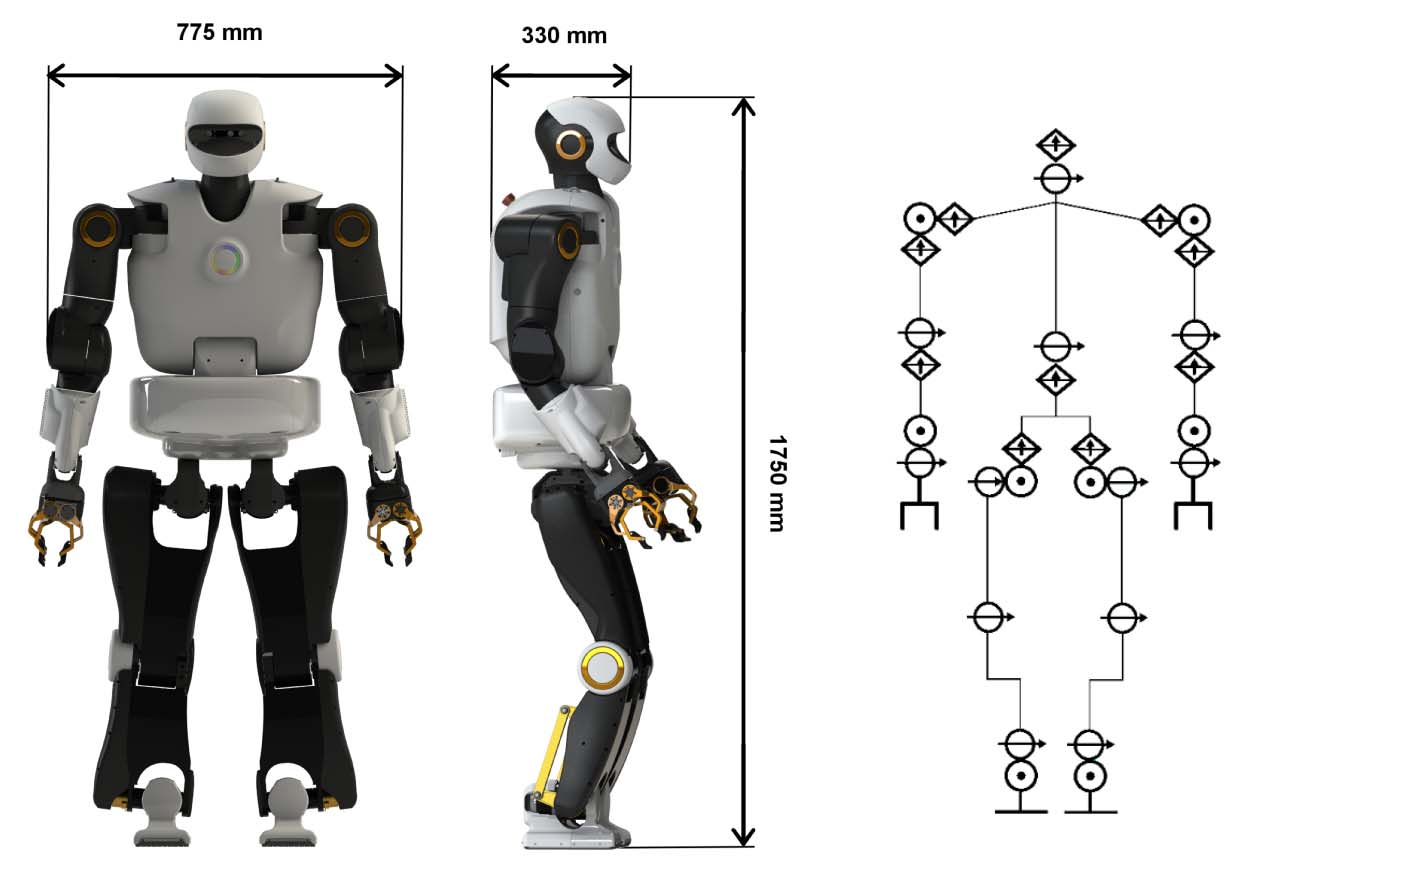
\includegraphics[width=\textwidth]{chapter_introduction/figures/talos_kinematics.png}
    \caption[Kinematics of Pyr\`{e}ne robot]{Kinematics of Pyr\`{e}ne robot. Image taken from~\citep{Stasse2017TALOS:Applications}    \label{fig:talos_kinematics}}
\end{figure}
\begin{figure}[tpb]
\centering
    \includegraphics{chapter_introduction/figures/talos_actuator.tikz}
    \caption{Structure of TALOS actuator \label{fig:talos_actuator}}
\end{figure}
\par
Figure~\ref{fig:talos_kinematics} presents the kinematics of Pyr\`{e}ne, which weights $\SI{95}{\kilo \gram}$ and is $\SI{1.75}{\meter}$ tall. It has $32$ actuated degrees of freedom in total and they are distributed as follows: $2$ joints in the head, $7$ joints in the arm, $3$ of which in the shoulder, $2$ in the elbow, and $2$ in the wrist, and $1$ joint in the gripper. $2$ joints allow controlling the pitch and yaw torso motion. Each leg has $6$ joints.
\par
Pyr\`{e}ne is equipped with Cobalt-Nickel-Manganese (Li-CNM) batteries that are capable of providing $\SI{75}{\volt}$ with a capacity of $\SI{15}{\ampere \hour}$. In the case a more power-consuming motion needs to be performed, the batteries can deliver current peaks of $\SI{150}{\ampere}$.
\par
Figure~\ref{fig:talos_actuator} presents the actuator structure of the TALOS robot. Each brushless DC motor is connected to a harmonic drive, which is attached to a torque sensor. The torque sensor is connected to a link.
Unlike iCub, each joint motor assembly is equipped with a torque sensor that can directly measure the torque applied on the load side. Furthermore, two high-precision encoders (19 bits each) measure the motor and joint positions.
Pyr\`{e}ne mounts an IMU at the level of its waist. This is involved in the estimation of the robot's base position and orientation. Similar to iCub, Pyr\`{e}ne is equipped with 6-axis force/torque sensors at the level of the hands and the feet. These sensors are often exploited to measure the contact force that the robot acts on the surrounding environment. 

\par
The robot comes with two processors, each with a dual i7 CPU running at 2.8 GHz. Each CPU contains two cores and is hyperthreaded, giving the machine a total of eight cores. 
The communication between the motors and sensors boards and the computers is implemented with an EtherCAT network~\citep{IEC61158-12019IndustrialSeries}. Because of TALOS' EtherCAT communication network, control loops can run at 2 kHz and up to 5 kHz, allowing for extremely reactive and dynamic motions.
\par
Pyr\`{e}ne runs Ubuntu 18.04 LTS as its operating system.
The ROS control system was used to develop the robot's low-level system.
The multimedia system uses stacks to provide navigation and map building. Furthermore, a complete Gazebo~\citep{Koenig04} simulation environment is provided.
\section{Notation}\label{sec:notation}
Throughout the thesis we will use the following notation.
\begin{itemize}
	\item The $i_{th}$ component of a vector ${x}$ is denoted as $x_i$. 
	\item The transpose operator is denoted by $(\cdot)^{\top}$.
	\item Given a function of time $f(t)$ the dot notation denotes the time derivative, i.e.
		$\dot{f} := \frac{\diff f}{\diff t}$. Higher-order derivatives are denoted by a corresponding amount of dots.
	\item $I_n \in \mathbb{R}^{n \times n}$ denotes the identity matrix of dimension $n$.
	\item ${0}_{n \times n} \in \mathbb{R}^{n \times n}$ denotes a zero matrix, while ${0}_n = {0}_{n \times 1}$ is a zero column vector of size $n$.
	\item ${e}_i$ is the canonical base in $\mathbb{R}^n$, i.e., ${e}_i = [0, 0, \dots, 1, 0, \dots, 0]^\top \in \mathbb{R}^n$, where the only unitary element is in position $i$. Throughout the thesis, $n$ will be 3 or 6 depending on the context. 
	\item The operator $\times$ defines the cross product in $\mathbb{R}^3$. 
	\item The weighted L2-norm of a vector ${v} \in \mathbb{R}^n$ is denoted by $\|{v}\|_{{\Gamma}}$, where ${\Gamma} \in \mathbb{R}^{n\times n}$ is a positive define matrix.
	\item $\mathcal{I} = (o_\mathcal{I}, [\mathcal{I}])$ is a fixed inertial frame with respect to (w.r.t.) 
	which the robot's absolute pose is measured. Its $z$ axis is supposed to point against gravity, while the $x$ direction defines the forward direction. $o_\mathcal{I}$ denotes the origin of the frame and $[\mathcal{I}]$ its orientation.
    \item Given the inertial frame $\mathcal{I}= (o_\mathcal{I}, [\mathcal{I}])$  and a frame $B= (o_B, [B])$, we define $B[\mathcal{I}] =(o_B, [\mathcal{I}])$ as the frame having its origin in $o_B$ and the orientation as the inertial frame. 
	\item $^{A}{R}_{B} \in SO(3)$ and $^{A}{H}_{B} \in SE(3)$ denote the rotation and transformation matrices that transform a vector expressed in the $B$ frame, $^B {x}$, into a vector expressed in the $A$ frame, $^A {x}$.
	\item ${}^D\mathrm{v}_{A,D} \in \mathbb{R}^6$ is the relative velocity between frame $A$ and $D$,  whose coordinates are expressed in frame $D$.
	\item ${}_D\mathrm{f}\in \mathbb{R}^6$ is the 6D force applied in $D$,  whose coordinates are expressed in $D$.
	\item ${x}_\text{CoM} \in  \mathbb{R}^3$ is the position of the center of mass relative to $\mathcal{I}$.
	
\end{itemize}
